\documentclass[twoside,11pt]{cergdoc}
\usepackage{graphicx}
\usepackage{amsmath}
\usepackage{listings}
\usepackage{longtable}

\newcommand\thead[1]{\multicolumn{1}{c}{\textbf{#1}}}
\newcommand\theadr[1]{\multicolumn{1}{c|}{\textbf{#1}}}
\newcommand{\ITwoC}{I\textsuperscript{2}C }


\begin{document}

\lstset{%
  basicstyle=\ttfamily,
  language=C,
  otherkeywords={bis.b,bis.w,bic.b,bic.w,bit.b,bit.w,mov.b,mov.w,dec.b,dec.w,jnz,jmp},
  commentstyle=\color{cerglightblue},
  keywordstyle=\color{cergpink},
  numberstyle=\color{cergpred},
  stringstyle=\color{cergblue},
  identifierstyle=\color{cergpurple}
}


\title{XXBX Device Under Test -- XBD}
\subtitle{XBD User Guide v1.0}
\author{Matthew R. Carter \and Raghurama R. Velegala \and Jens-Peter Kaps}
\email{jkaps@gmu.edu}
\affiliation{George Mason University\\
  Fairfax, Virginia}
\topicpic{xxbx-slide}

\maketitle

\tableofcontents

% -----------------------------------------------------------------------------
\chapter{Introduction}
% -----------------------------------------------------------------------------
XBD has two main software components: the Bootloader and
the Application. It is initially flashed with the Bootloader, which
contains the Hardware Abstraction Layer and can perform
rudimentary functions such as initializing the I2C module,
Clocks module, GPIO ports, Universal Serial Communication
Interface (USCI), etc and also be able to report timing
measurements for calibration and receive the Application over
I2C.
On the other hand, the Application contains the wrapper for the
algorithm and helper functions to set up the stack, parameters to
be used by the algorithm, and to signal execution to the XBH.
The RAM usage is measured by the Application by counting the
available stack and painting it with Canaries, executing the
algorithm, and then reading the stack again to see how much
memory has been used.






The XBD software remained largely identical to that in original XBX. Most of the
changes were limited to refactoring or adding AEAD support. 

The substantially more comprehensive self-test suite to verify correctness of
the primitive implementations from SUPERCOP replaced the simplified version
found in XBX, as we wanted to retain this aspect of SUPERCOP and did not want to
write our own test for AEAD. 

Unfortunately this leads to substantially longer
execution times and precludes operation with smaller devices especially for
AEAD, which was probably the original XBX team's motivation for writing a
simplified check. 

For AEAD, the test requires two large buffers, one for input ciphertext/auth data and
one for output, and multiple smaller buffers for keys, secret number,  as
opposed to hash functions, which only need a large buffer for the input and a
substantially smaller buffer for the hash, with the largest output being 512
bits (64 bytes). In addition AEAD primitives require
multiple smaller buffers for various parameters defined in the CAESAR interface,
each with padding in order to detect overruns. The buffers and limits we
assigned for AEAD are:
\begin{itemize}
    \item Message
    \item Associated Data (Associated Data+Message must be less than 2048 bytes)
    \item Ciphertext, which is the size of Message+Associated Data plus additional bytes for
        authentication. Additional bytes is limited to 128 bytes.
    \item Secret Bytes (64 bytes)
    \item Public Bytes (64 bytes) 
    \item Key Bytes (64 bytes)
\end{itemize}

Some primitives had unreasonable sizes for parameters such as Trivia-128v1 which
specified slightly over 512kiB of additional bytes to the output, which is well
over the total memory of most microcontrollers We decided on these limits since
we deemed them the maximum reasonable for an embedded platform, although we
leaned towards larger sizes unlikely to be found in an embedded environment in
order to include more primitives. Embedded devices might also use larger than
ideal primitives for interoperability reasons.

Other aspects of the XBD code were also modified to make most of the XBD code as
operation-agnostic as possible, except for the test code. References to hash
functions were removed in code that was generic to all operations. 

In order to support a new operation already supported by SUPERCOP, changes are
limited to modifications to the script used to generate the tests in order to
allocate memory in order to fit our more restricted framework and code to unpack
message payloads to set the appropriate buffer pointers.

%----- merge above (John) with below (Girmay)



The software for the XBD is largely the same
as the original XBX. Self-test implementation was
replaced with SUPERCOS's (?). The XBD
software factored out hash-specific code to
make it easier to add other operations. There
was added a AEAD payload processing.
XBH doesn't know anything about the
operation under test, just routes it blindly to
XBD from XBS. XBD must know what is
being in run order to unpack
parameters and messages
The XBD code consists of a small
bootloader that is flashed once to XBD that
performs basic calibration and selfprogramming
of the primitive
implementations over the communications
channel. After that, application download
and execution is handled over a
communication channel established between
the bootloader and the benchmarking
harness.

% -----------------------------------------------------------------------------
\chapter{Hardware Abstraction Layer}
% -----------------------------------------------------------------------------
% -----------------------------------------------------------------------------
\chapter{Boot Loader}
% -----------------------------------------------------------------------------
  \section{Overview}
The bootloader for the XBD is
located in xbs\_xbd/embedded/xbd\_bl.c. It is
compiled with HAL and its operation for
XBH to XBD communication is highlighted
in xbs\_xbd/embedded/xbd\_app.c. There’s
some utilities defined in
xbs\_xbd/embedded/xbd\_af.c. The operations
and hash to use are located in
xbs\_xbd/embedded/xbd\_op.c. Bootloader
can be debugged using console on XBD.

  \section{Stack Usage Measurement}
The HAL contains two functions that
allow for stack measurement: paintStack and
countStack. PaintStack ’paints’ the free
stack area with a known pattern, called a
canary bird. Then the function to be
benchmarked is called and after it returns,
countStack counts the number of canary
birds that did not ’survive’. This gives the
maximum amount of stack used by the
benchmarked function. Combined with the
static RAM requirement obtained from the
application binary and the known RAM
requirement of the AF, the total RAM
consumption of a triple [Algorithm,
Compiler, Options] can be measured.
The file
embedded/xbd/xbd\_op/crypto\_aead/XBD\_O
H.c provides a means to measure the stack
usage. The steps are as such, paint stack, run
code, check stack, report to XBD. There is
also apparently a size command that gets the
ROM usage and RAM usage.


  \section{XBH-XBD Communication}
    \subsection{\ITwoC Interface}
    \subsection{XBH-XBD Protocol}
Much of the core XBH code dealing
with the XBH <-> XBD protocol and packet
formats was reused, with some rewriting to
conform to preferred coding conventions,
such as using C99 inttypes.h instead of
custom typedefs. From XBH command was
sent in such a way as to contain the opcode
and the CRC value. Then XBD responded
by sending back the command plus the data
and the 2 byte CRC value. Some of the
possible commands are XBD04SBR for
properly starting bootloader, and
XBD04TCR for timing calibration request.
There’s many more defined in the codebase.



    \subsection{General Purpose IO}
    \subsection{Reset}
    \subsubsection{Debug}
The XBDs also contain UART debug interface that can be used
to test functionality of the program. Part of work also involved
fixing the debug interface on the original MSP30 XBD. An
important learned lesson here is that turning on the specific
debugging output resulted in execution delays which affected
the functioning of the system and caused errors related to I2C
communication.


% -----------------------------------------------------------------------------
\chapter{Application}
% -----------------------------------------------------------------------------
% -----------------------------------------------------------------------------
\chapter{Board Specific Changes}
% -----------------------------------------------------------------------------
  \section{TI MSP430F5529 LaunchPad\texttrademark}
Much of our previous work on original XBX for the MSP430FG4618 was reused, and
the work was mostly altering pinouts and adapting to the new MSP430-GCC
\cite{msp430-gcc} toolchain, which had substantial differences to the older
MSPGCC toolchain \cite{mspgcc}.

We decided to clock the MSP430F5529 at 16MHz, matching the clock rate on the AVR
platforms in original XBX. The clock initialization on the MSP430F5529 is more
complicated, and we used code from the Energia \cite{energia} project to handle
this. The digitally controlled oscillator (DCO) in the MSP430F5529 does not run
at exactly 16MHz, but mixes two frequencies to get an average at the specified
frequency. This causes jitter and has implications for accurate measurement when
cycles are measured externally, however the impact is likely to be negligible
for the purpose of comparing algorithms. This is a motivation for using cycle
counters where available if more precise measurements are needed, however.

In order to support LTO, we had to mark the interrupt handler for resetting the
XBD explicitly as used using GCC attributes. Attributes are a compiler-specific
C extension used to apply a property to a C function or variable, that is not in
standard C. Without this attribute, LTO would optimize out the interrupt
handler.

  \section{TI MSP430FR5994 LaunchPad\texttrademark}
Another significant aspect for the XBDs in general is their
placement of the Bootloader and the Application in their flash
memory. More specifically regarding MSP430FR5994, the
memory is organized as follows.

    \subsection{Memory Map}
fig is in 746-paper.

As we can see from the memory organization, the interrupt
vector is placed in the Flash memory and so the memory is not
contiguous. Currently the bootloader is being placed at address
0xE810 which leaves 6k for the bootloader, the Applicationloaded to 0x4000 which means its size can be 43024 bytes.future improvement here would be to place the bootloaderHIGH FRAM and leave the full 49k LOW FRAM for only the
Application. This would allow for heavier sized algorithms tobenchmarked. This restriction also limited the size of the
algorithms that could be run on this XBD (discussed later in the
Results section).

MSP430FR5994 (the new XBD) is similar to MSP430F5529
(original XBD) however there were some changes that needed to
be accounted for.

One of them was the standardization of the 16-bit
control registers as opposed to the 8-bit registers in the
original XBD and changes in some register naming
conventions.
The clocks system module on the new XBD allows for
only specific discrete frequencies but the original XBD
used a programmable multiplier to allow for more
selectable range of frequencies.
The original XBD used a 32-bit register (2 16-bit
concatenated registers) in the RTC for busy looping for
1 sec. during timing calibration. This was not possible
on the newer XBD since the RTC no longer allowed for
concatenating two registers and the module could not
source from the system clock (only a fixed 32KHz
clock). The solution for this was to use a Timer sourced
from the system clock with a wrap around interrupt.
Usage of interrupts is okay here since timing
calibration is done in the bootloader mode and not
during algorithm execution.
The timing calibration measurements are only done to check if
the XBD is running at the set frequency. The actual execution
times however are measured by the XBH using its own 120
MHz timer to be consistent with other XBDs timing
measurements.

    \subsection{Flash}
    \subsection{Using AES Peripherals}
Most of the algorithms have AES as their underneath function
during encryption and decryption. Some of them use total AES
encryption, some others use single round AES and some others
single round AES without XOR of key.

Fig 6. Functions in AES Rounds

To do the above implementation of the AES the algorithm has a
software implementation of AES which does all the functions in
a similar way mentioned below
KeyAddition(a,rk[0],BC);
for(r = 1; r < ROUNDS; r++) {
Substitution(a,S,BC);
ShiftRow(a,0,BC);
MixColumn(a,BC);
KeyAddition(a,rk[r],BC); }
Substitution(a,S,BC);
ShiftRow(a,0,BC); KeyAddition(a,rk[ROUNDS],BC);
While implementing algorithm on the microcontroller it runs a
AES program that has the above programs, on MSP430-5529
while the algorithms are implemented during both encryption
and decryption the program is called and AES implementation is
done. The same can be done with MSP430-5994 as well but
main advantage with this microcontroller is it has in built AES
accelerator which can be utilized instead of the software AES
implementation.

figs in 746 paper

The AES accelerator is present in some of the microcontrollers
like MSP-430 5994 which performs the both AES encryption
and decryption of 128 bit message data with different sizes of
the key(128, 192 , 256bits) that is given to it.
AES accelerator has different features:
- AES encryption for 128 bit can be done in 168 cycles,
192 bit in 204 cycles, 256 bit in 234 cycles.
- AES decryption can be in a similar fashion as
encryption but for only 192 bit it takes 206 cycles.
- Key expansion for encryption and decryption can be
done on the fly.
- Key generation for decryption can be offline.
- DMA support for ECB, CBC, OFB, and CFB cipher
modes.
- The input data, output data and key can be accessed
either as byte or word. But the issue is we can not mix
both word and byte access during the time of reading or
writing the data to the registers.
- AES ready interrupt flag.

Registers in the block diagram:
AESADIN, AESAXDIN: The data that needs to go in
to the AES module as input is given into this registers.
AESAKEY: The cipher key given is loaded into this
register.
AESADOUT: The output can be read out from here.
Encryption in Accelerator: The plain text that is given in the
AESADIN in subjected to rounds of transformations along with
using the key located in AESAKEY and then the ciphertext is
produced at the AESADOUT.
Decryption in Accelerator: AESAXDIN now has the ciphertext
which is subjected to rounds of transformations along with the
cipher key that is available at AESAKEY and then plain textproduced at the AESADOUT.




  \section{TI MSP432P401R LaunchPad\texttrademark}
  \section{TI Stellaris\textregistered~LM4F120 LaunchPad}
Much of the work assembling the toolchain, sorting out platform quirks, and
sorting through licensing on the TM4C1294 XBH applied to the TM4C123.

Open On-Chip Debugger (OpenOCD) is a tool used to program and debug various
chips and boards, including the Tiva-C boards used as the XBH and an XBD
\cite{openocd}. Currently, it does not support multiple Texas Instruments
In-Circuit Debug Interface (TI-ICDI) attached to the
same PC. We wrote a patch \cite{openocd_patch} in order to distinguish different
TI-ICDI devices by serial number. 

We encountered some issues programming the primitive implementations into the
XBD. The IHEX files containing the code to be downloaded to the XBD contained holes, which
are unused memory areas that are not specified in the file, making the defined
memory locations noncontiguous. The original XBS software did not properly take
these into account, and would load nonadjacent blocks of code adjacently. This
was fixed in the XBS rewrite. 

  \section{TI Tiva\texttrademark~C Series EK-TM4C123GXL LaunchPad}
For accurate power measurements remove the jumper near R30 shown next to the letter B in Fig.\,\ref{fig:tm4c123-power}. 
Then carefully cut the trace from the first pin of J1 marked with the letter A in the figure near J3 and R29.
The trace is highlighted in light pink and the point to cut indicated with a blue line.
Make sure to only cut the trace and not the surrounding traces (i.e. don't make a cut that is as long as
the blue line.) Place a jumper cable from point A to point B to power the board through the 
BoosterPack connector. The in-circuit-debugger-interface (ICDI) will not be powered. 
The setting of the power select switch has no influence on the measurements.

When programming the board using the ICDI, simply disconnect the board from the XBP and close the jumper
near R30. The cable to Pin 1 of J1 (marked with A in the figure) has to be removed and that pin 
will not be powered. Make sure that the power select switch is set to \emph{DEBUG}.

\begin{figure}[ht]
  \begin{center}
    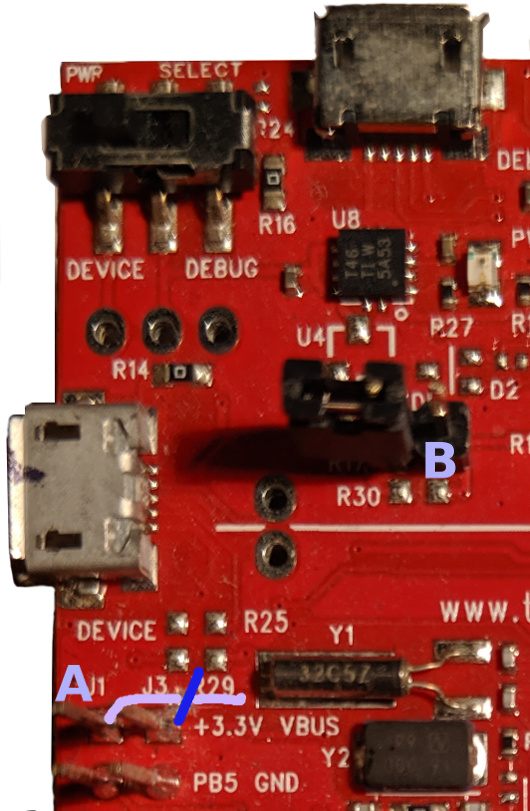
\includegraphics[scale=0.3]{figures/ek-tm4c123gxl-power}
    \caption{Modifications of the EK-TM4C123GLX LauchPad for Power Measurements}\label{fig:tm4c123-power}
  \end{center}
\end{figure}


  \section{TI Tiva\texttrademark~C Series EK-TM4C129EXL LaunchPad}
Remove jumper JP3 in order to power the XBD through the BoosterPack header from the XBP.
Then connect the BoosterPack1 header to the XBP. More information on how to enable precise power measurements
will follow soon.

  \section{ST Microelectronics NUCLEO Boards}
% -----------------------------------------------------------------------------

% -----------------------------------------------------------------------------
\begin{appendix}
\chapter{XBH - XBD Protocol}
%\begin{table}\centering%
  \begin{longtable}{llll}
    \caption{Commands of the XBH --- XBD Protocol}\label{tab:xbh-xbd} \\ \hline
    \endfirsthead
    \caption{(continued)} \\ \hline
    \endhead
      \multicolumn{2}{c}{\textbf{Requests understood by bootloader}} & \multicolumn{2}{c}{\textbf{Responses}}\\ 
      \thead{CMD} & \thead{Functionality}               & \thead{OK} & \thead{Failed} \\ \hline 
      XBDpfr & Program Flash Request                        & XBDpfo & XBDpff \\
      XBDfdr & Flash Download Request                       & XBDpfo & XBDpff \\
      XBDsar & Start Application Request                    &        &        \\
      XBDvir & Version Information Request                  & XBDblo &        \\
      XBDtcr & Timing Calibration Request                   & XBDtco &        \\
      XBDtrr & Target Revision Request                      & XBDtro &        \\
      XBDlor & LOopback Request                             & XBDloo &        \\ \hline

      \multicolumn{2}{c}{\textbf{Requests understood by AppFramework}} & \multicolumn{2}{c}{\textbf{Responses}}\\ 
      \thead{CMD} & \thead{Functionality}               & \thead{OK} & \thead{Failed} \\ \hline 
      XBDppr & Program Parameter Request                    & XBDppo & XBDppf \\
      XBDpdr & Program Download Request                     & XBDpdo & XBDpdf \\
      XBDurr & Upload Result Request                        & XBDuro & XBDurf \\
      XBDrdr & Result Data Request                          & XBDrdo & XBDurf \\
      XBDexr & EXecute Request                              & XBDexo & XBDexf \\
      XBDccr & Checksum Compute Request                     & XBDcco & XBDccf \\
      XBDsbr & Switch to Bootloader Request                 &        &        \\
      XBDvir & Version Information Request                  & XBDafo &        \\
      XBDtcr & Timing Calibration Request                   & XBDtco &        \\
      XBDsur & Stack Usage Request                          & XBDsuo &        \\ \hline
      
      \multicolumn{2}{c}{\textbf{Common Responses}}         &        &        \\ 
      \thead{CMD} & \thead{Functionality}                   &        &        \\ \hline 
      XBDunk & UNKnown command                              &        &        \\ 
      XBDcrc & CRC error                                    &        &        \\
      XBDfdo & -- Not Used --                               &        &        \\
      XBDfdf & -- Not Used --                               &        &        \\ \hline
      
  \end{longtable}
%\end{table}

\end{appendix}


\end{document}
